% slides.tex
\documentclass{beamer}
\usetheme{default}
\usepackage[absolute,overlay]{textpos} 
\newenvironment{reference}[2]{% 
  \begin{textblock*}{\textwidth}(#1,#2) 
      \footnotesize\it\bgroup\color{red!50!black}}{\egroup\end{textblock*}} 

\title{Detecting Snow Cover on GPS Antenna}
\subtitle{ASEN6090 Final Project}
\author{Kyle Wolma\\Logan Finch\\Praveen Vikram\\}
\institute[CU-ASEN]{
  Department of Aerospace Engineering Sciences\\
  Colorado University\\
  \texttt{kyle.wolma@colorado.edu\\logan.finch@colorado.edu\\praveen.vikram@colorado.edu}
}
\date[May 2012]{May 04, 2012}

\begin{document}

%--- the titlepage frame -------------------------%
\begin{frame}[plain]
  \titlepage
\end{frame}

%--- outline frame -------------------------%
\begin{frame}{Outline}

\begin{itemize}
  \item Goals
  \item Sites 
  \item Model
  \item MP$_1$ Results
  \item SNR Results
  \item Position Results
  \item Conlusions
\end{itemize}

\end{frame}

\begin{frame}{Goals}
\begin{itemize}
  \item Generate an index representative of snow cover over GPS antenna.
  \item Considerations for Reflections study:
  \begin{itemize}
    \item How much of an effect will Snow cover directly over the antenna have on received signal power from lower elevation angles.
%    \item Ice may form on the side of antenna, which may cause problems.
%    \item Detect signal loss from archived direct signal power for each SV at binned elevation.  
  \end{itemize}
\end{itemize}
\end{frame}

%--- sites frame -------------------------%
\begin{frame}{Sites}

Sites for Primary Study
\begin{itemize}
  \item P360 *
  \item P101 *
  \item AB33
  \item P455
\end{itemize}

   \begin{reference}{4mm}{85mm}
     * sites have a digital camera installed on site.
   \end{reference} 
 
\end{frame}

\begin{frame}{Model}
\begin{itemize}
\item Basic EM wave propogation (Plane solution to Maxwell's Equations)
  \begin{equation}
    E = E_0e^{j(k.r -\omega t)},
  \end{equation}
  Where,
  \begin{equation*}
    \frac{\omega^2}{k^2}=\frac{c^2}{\epsilon}
  \end{equation*}
  However, If $\epsilon$ is complex
  \begin{equation}
    E = E_0 exp[j (Re(k).r - \omega t)]exp[-Im(k).r].
  \end{equation}
\end{itemize}
\begin{center}
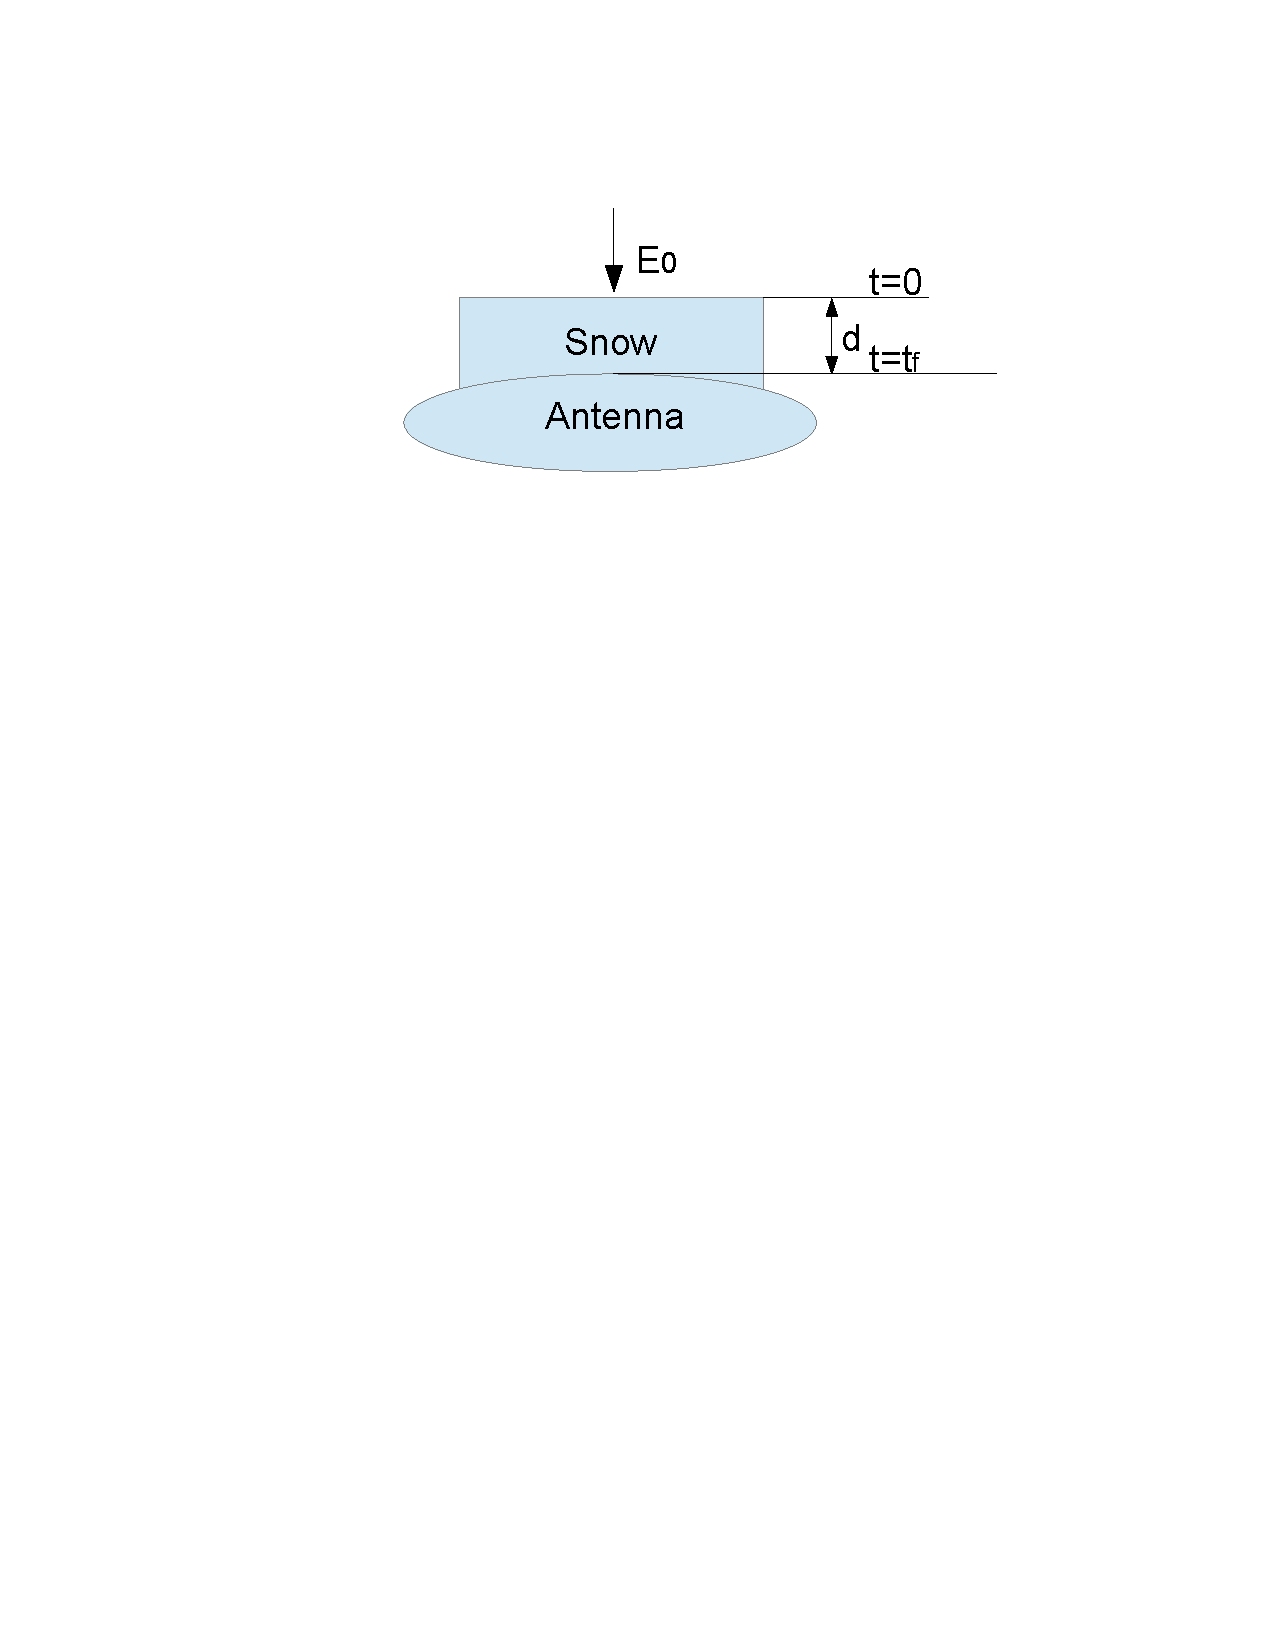
\includegraphics[width=0.8\linewidth,trim=100 100 100 100, clip=true]{model1.pdf}
\end{center}
\end{frame}

\begin{frame}{Model}
\begin{itemize}
  \item Dielectric of Snow?
    \begin{itemize}
      \item Phase velocity in a medium is dependent on the frequency of the wave-front.
      \item As a consequence the dielectric constant of a medium is dependent on the frequency of the EM-wave.
      \item Phase velocity of the wave is given by
        \begin{equation*}
          v = \frac{\omega}{k} = \frac{c}{n}
        \end{equation*}
        Where, $n$ is the refractive index of the the medium
        \begin{equation*}
          n = \sqrt{\epsilon}
        \end{equation*}
    \end{itemize}
    \item Dielectric of Snow for GPS L1 frequency?
\end{itemize}
\end{frame}

\begin{frame}{Model - $\epsilon$ for Snow}
\begin{itemize}
  \item Snow is a mixture of Ice, Air and Water.
  \item From [1]
    \begin{itemize}
      \item Consider a 2 component mixture: ice and air
      \item Let their volume fractions be $p_i$ and $p_a=(1-p_i)$
      \item let their dielectric constants be $\epsilon_i$ and $\epsilon_a$
      \item The Dielectric constant of the combination is given by,
        \begin{equation}
          \epsilon_s E_S = \epsilon_i p_i E_i + \epsilon_a p_a E_a
        \end{equation}
      \item Where $E_s$, $E_i$ and $E_a$ is the mean electric field strength for the EM wave under consideration in the different media.
    \end{itemize}
\end{itemize}

\begin{reference}{4mm}{85mm}
  [1] Y. Ozawa and D. Kuroiwa, "Dielectric Properties of ice, snow and supercooled water" in Microwave propogation in Snowy districts, no. 6, pp. 31-71, 1971
\end{reference}

\end{frame}


\begin{frame}{Model - $\epsilon$ for Snow}
\begin{itemize}
  \item From [2] 
    \begin{itemize}
      \item The Dielectric constant of the combination is given by,
        \begin{equation*}
          \epsilon_s = \epsilon_s'  - j\epsilon_s''
        \end{equation*}
        Where
        \begin{equation*}
            \epsilon_s' = 1 + 2 \rho_d
        \end{equation*}
        \begin{align*}
          \epsilon_s'' = &\epsilon_s' \times 1.59 \times 10^6 \times \frac{0.52\rho_d + 0.62\rho_d^2}{7 + 1.7\rho_d + 0.7\rho_d^2}\\
          & \times (f_{L1}^{-1} + 1.23 \times 10^{-6}\sqrt{f_{L1}})e^{0.036 T}
        \end{align*}
      \item Where, \\$\rho_d$ is relative density of dry snow \\$T$ is the temperature of snow in Celsius.
    \end{itemize}
\end{itemize}

\begin{reference}{4mm}{85mm}
 [2] M.E. Tiuri, A.H. Sihvola, E.G. Nyfors, M.T. Hallikaiken, "The complex dielectric constant of snow at microwave frequencies'', IEEE J Ocean. Eng. OE-9 (5), pp. 377-382, 1984
\end{reference}

\end{frame}

\begin{frame}{Model}
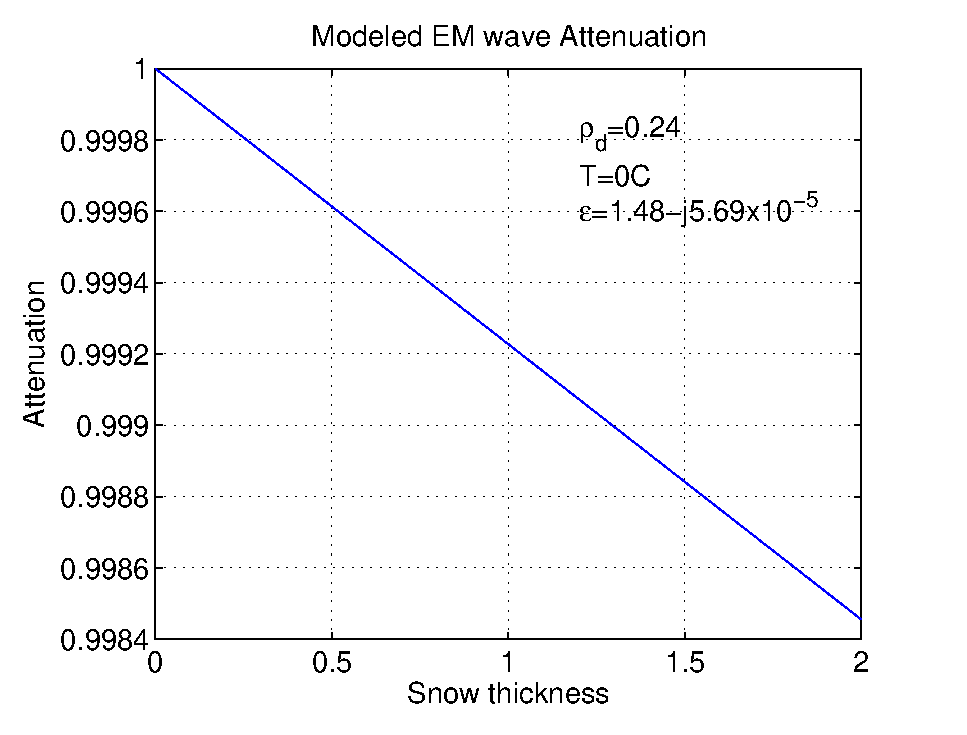
\includegraphics[width=1\linewidth]{model_1.eps}
\end{frame}

%%% Kyle's slides


%%% SNR slides
\begin{frame}{SNR}
  \begin{itemize}
  \item Generate a statistical map if expected SNR values w.r.t Elevation angle.
  \item Data from 2011 DOY 200-250 was used to generate the map
  \item Each SV was considered seperately
    \begin{itemize}
    \item Individual Tracks could be tagged as 'Bad'
    \item Each SV has varying transmit power
    \end{itemize}
  \end{itemize}
\end{frame}

\begin{frame}{SNR Map}
  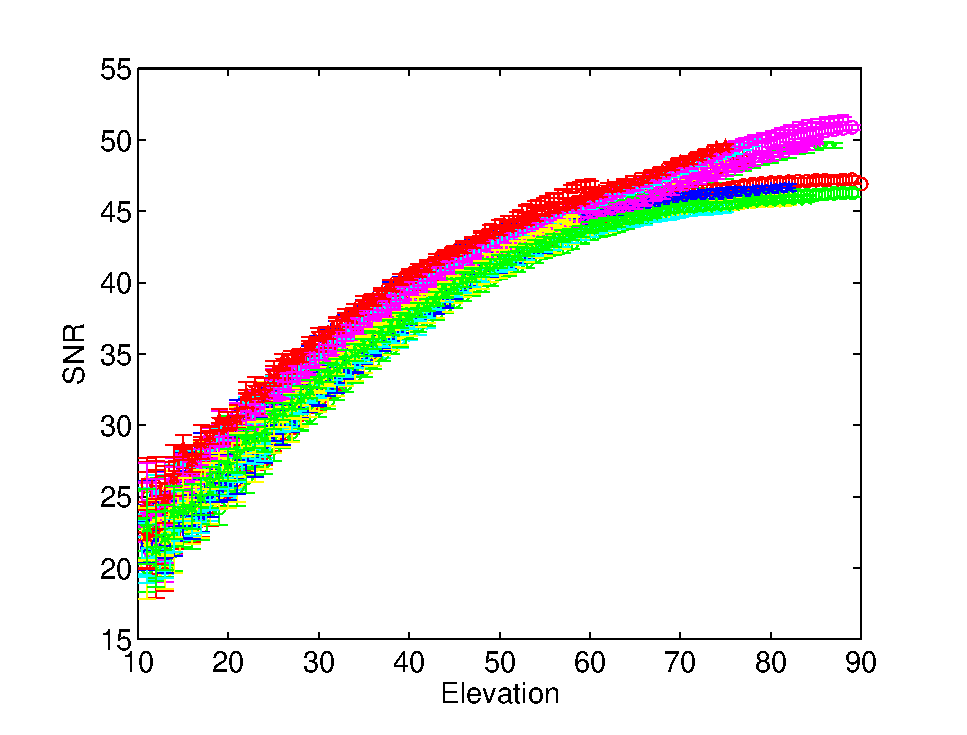
\includegraphics[width=1\linewidth,clip=true]{snrMap.eps}
\end{frame}

\begin{frame}{SNR Index}
  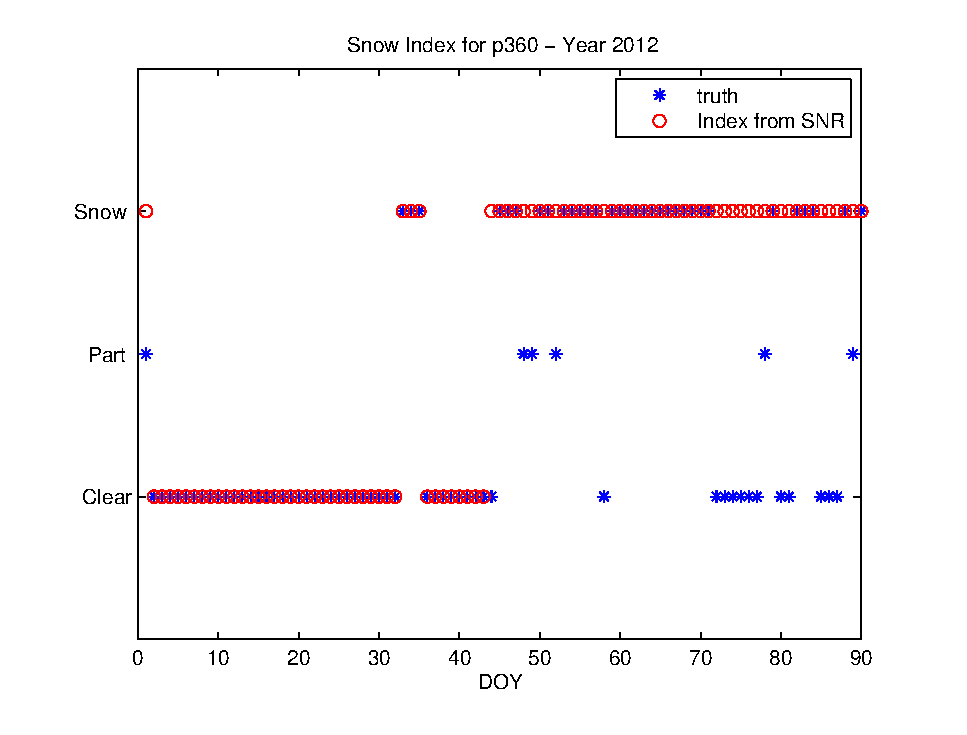
\includegraphics[width=1\linewidth,clip=true]{snrIndex.eps}
\end{frame}

%%% Logan's Slides
\begin{frame}{Position Time Series - P360}
  \begin{itemize}
  \item 2009 to 2012\\
  \end{itemize}

  \begin{columns}
    \column{.5\textwidth}
    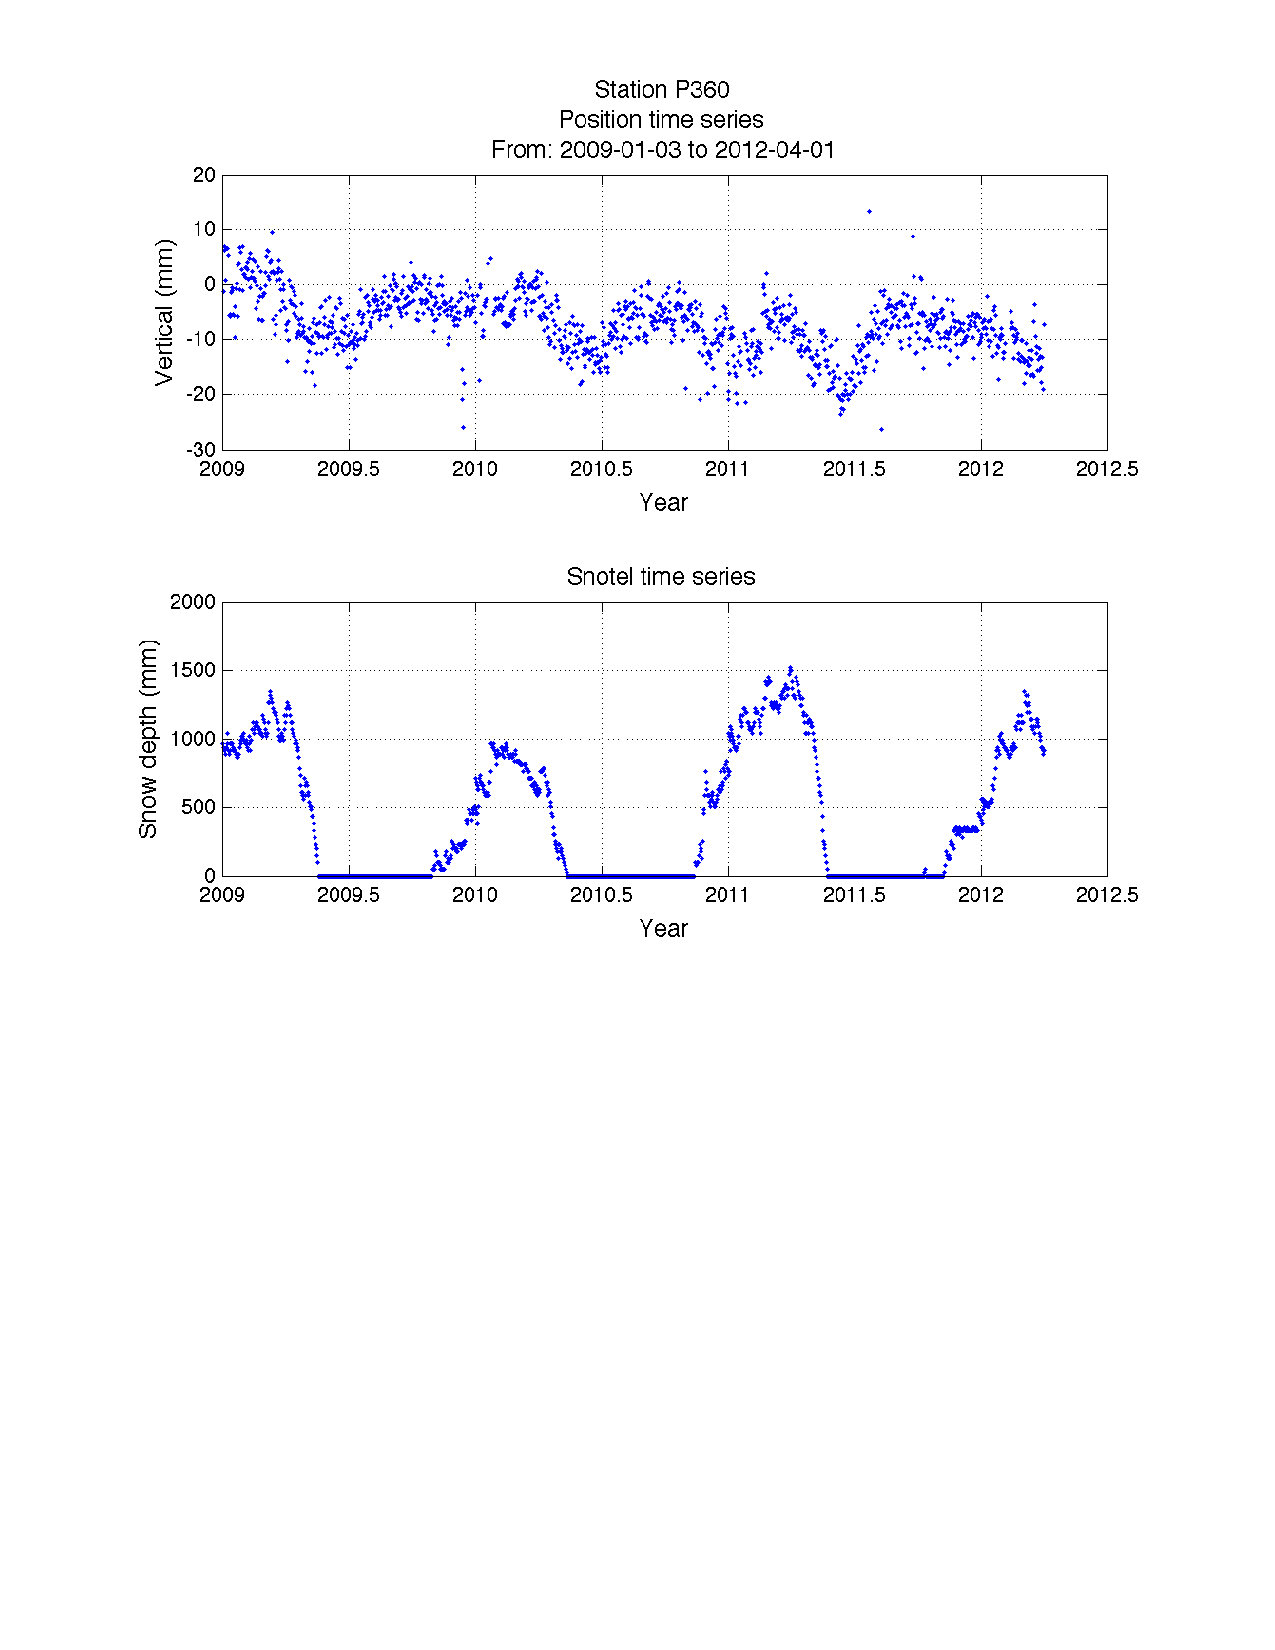
\includegraphics[width=1\linewidth,trim=70 300 70 50, clip=true]{logan/p360_pos.pdf}

    \column{.5\textwidth}
    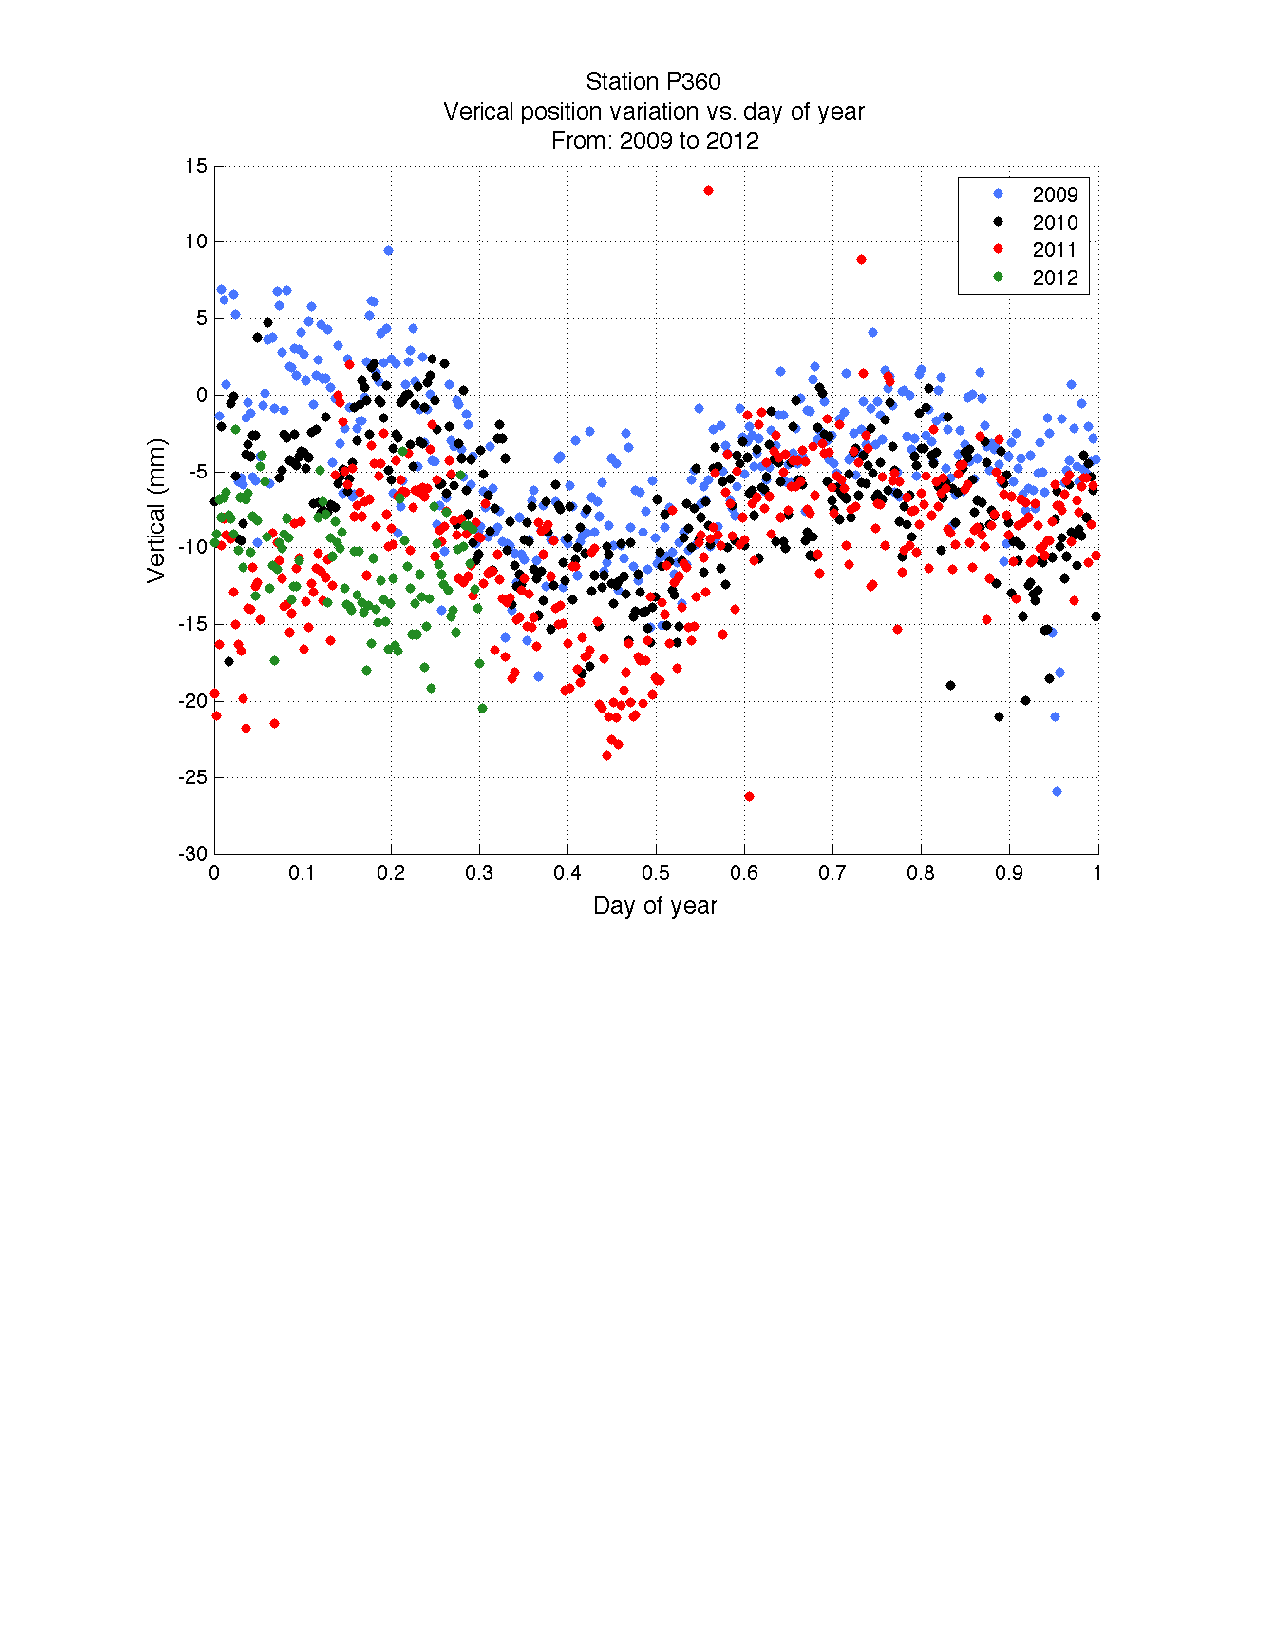
\includegraphics[width=1\linewidth,trim=70 300 70 50, clip=true]{logan/p360_pos_byYear.pdf}
  \end{columns}
\end{frame}

\begin{frame}{Position Time Series - P360}
  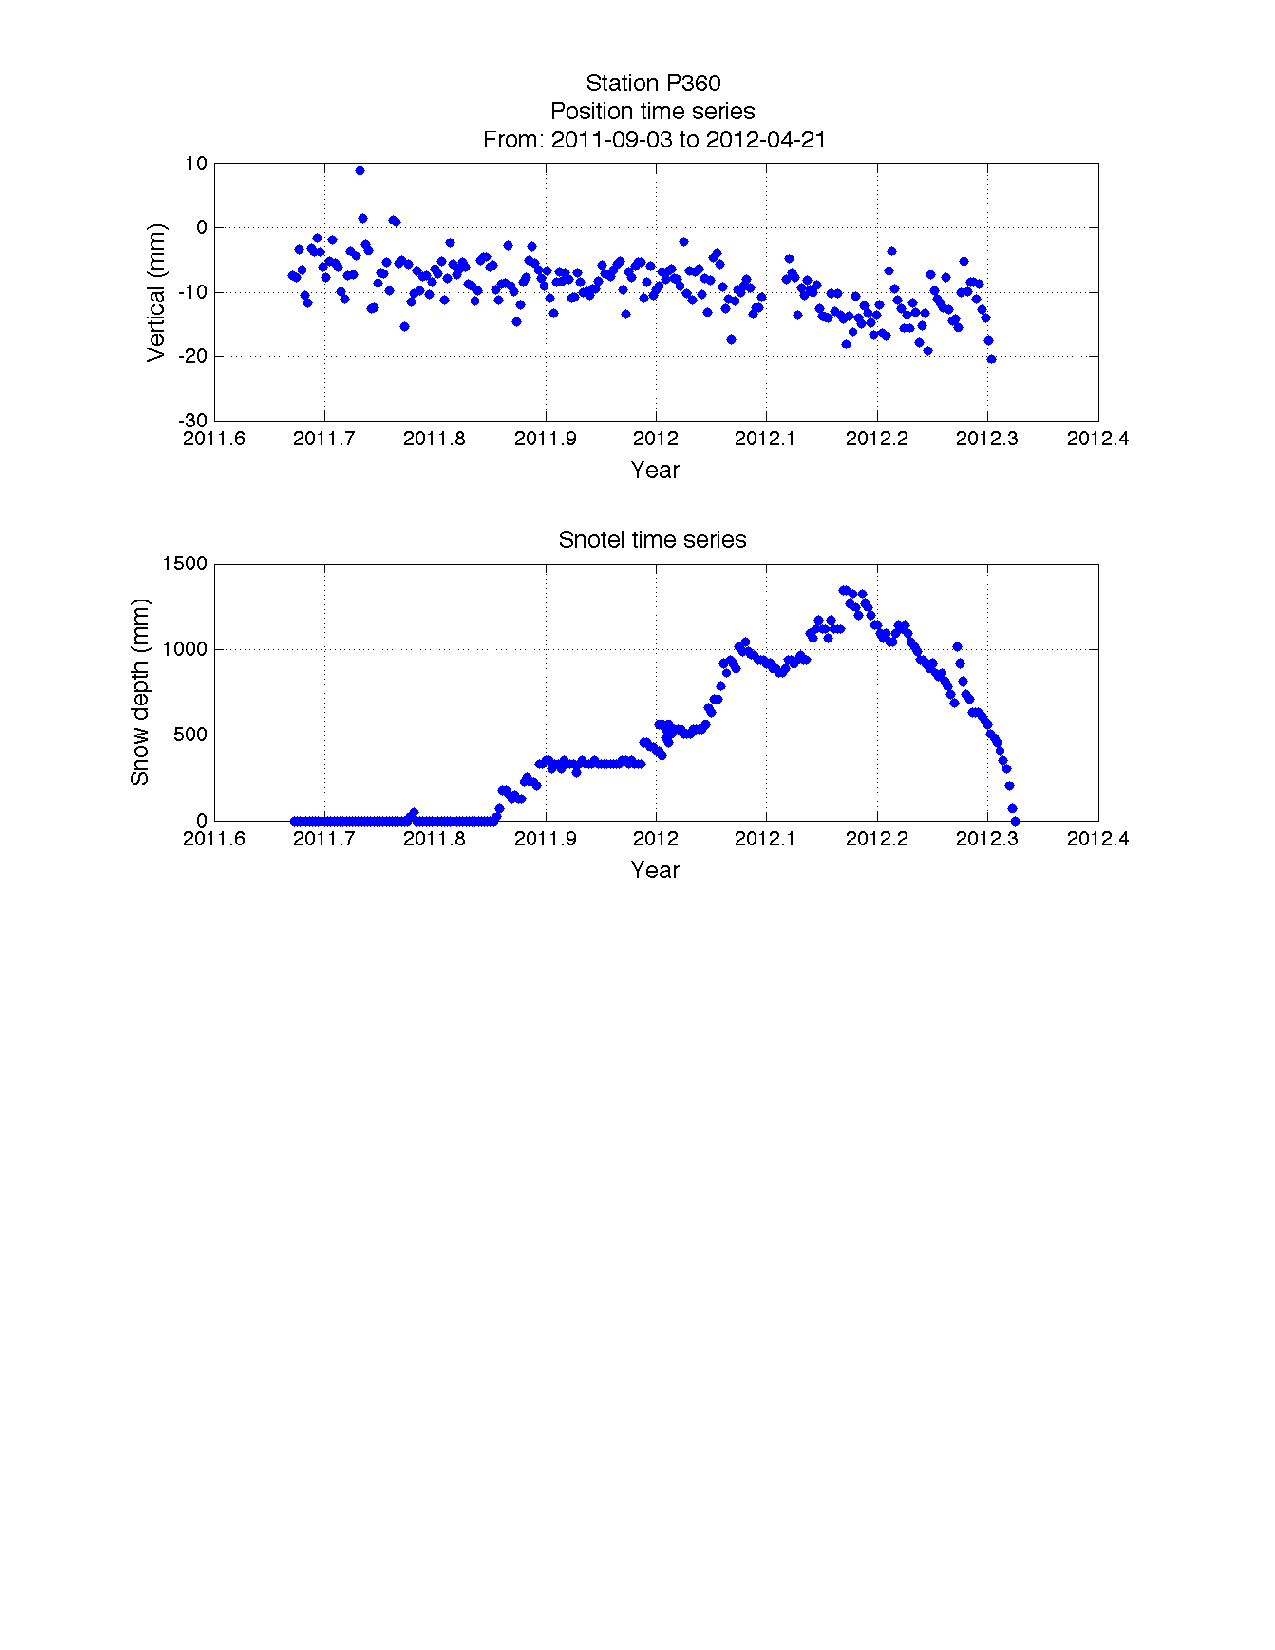
\includegraphics[width=1\linewidth,trim=50 0 50 20, clip=true]{logan/p360_snotel.pdf}
\end{frame}

\begin{frame}{Position Time Series - AB33}
\begin{itemize}
\item 2009 to 2012\\
\end{itemize}

\begin{columns}
\column{.5\textwidth}
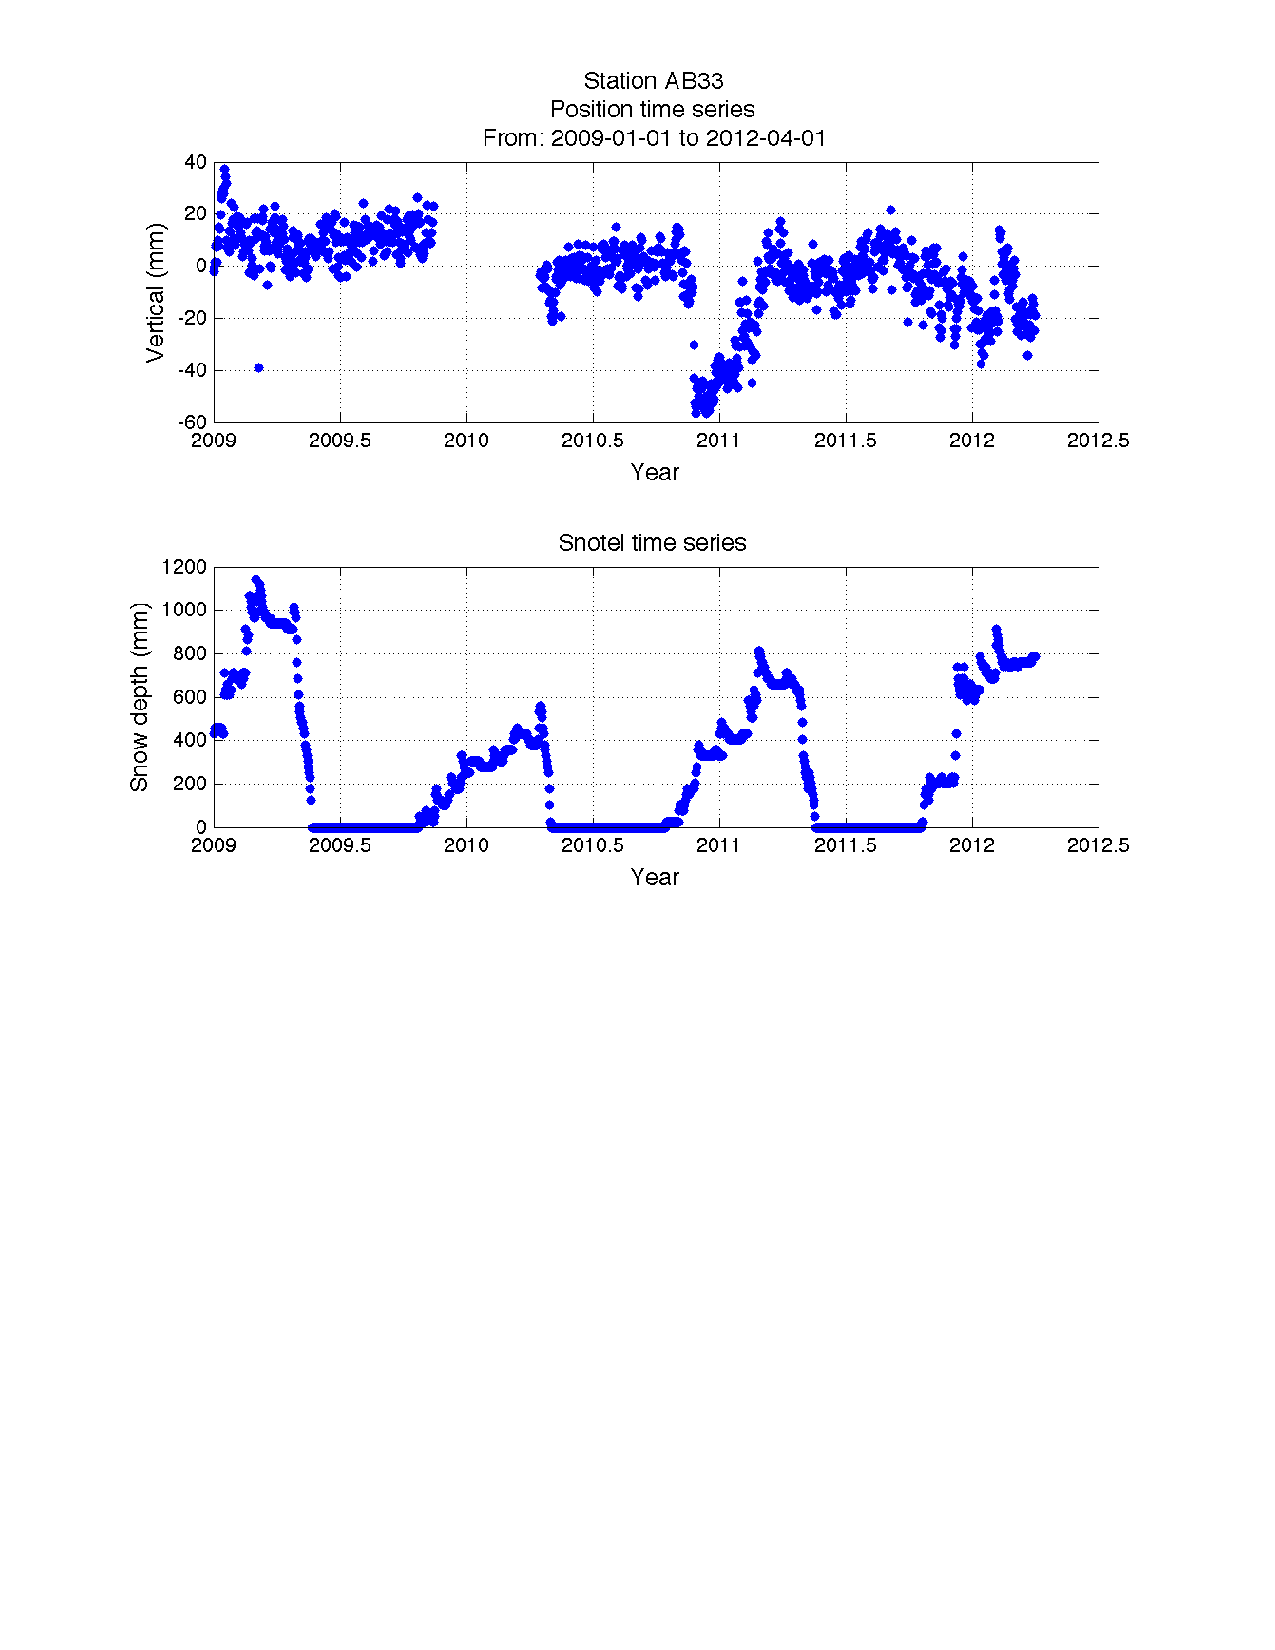
\includegraphics[width=1\linewidth,trim=70 300 70 50, clip=true]{logan/ab33_pos.pdf}

\column{.5\textwidth}
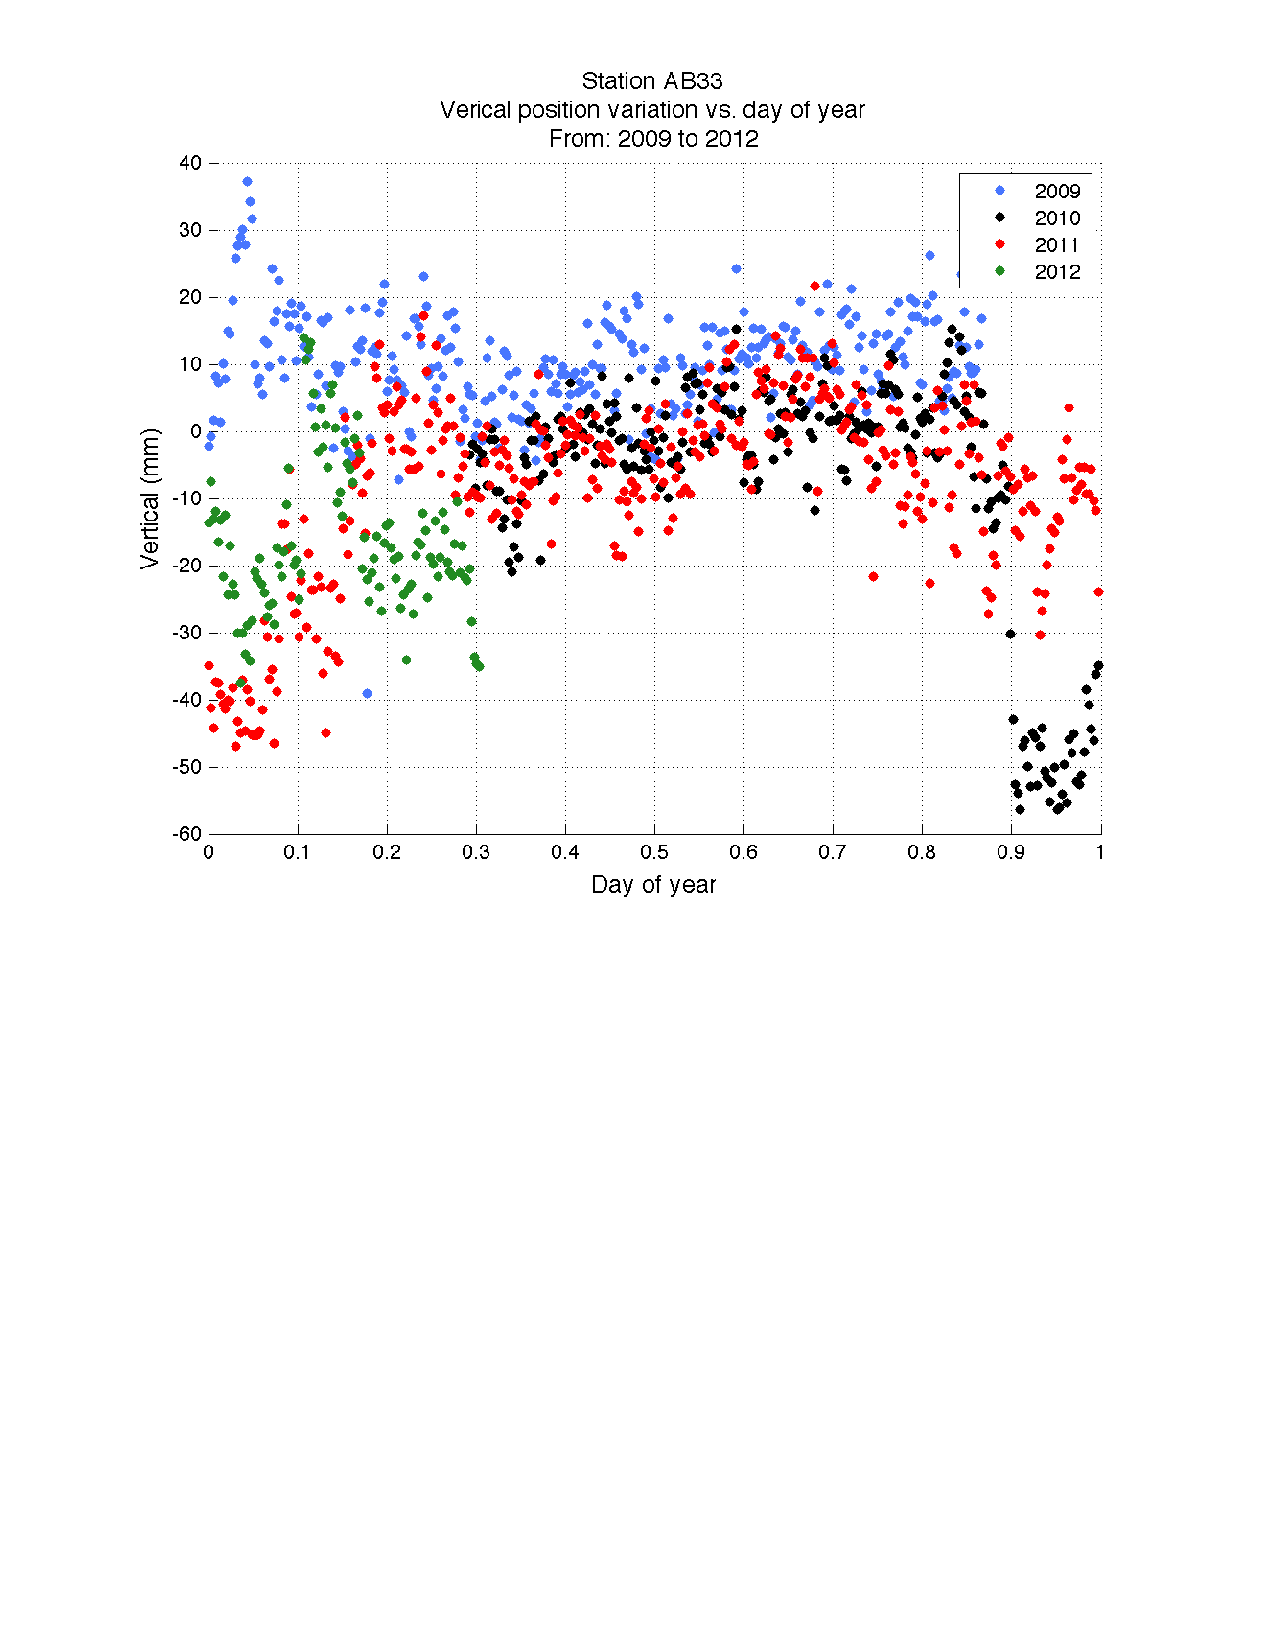
\includegraphics[width=1\linewidth,trim=70 300 70 50, clip=true]{logan/ab33_pos_byYear.pdf}
\end{columns}
\end{frame}

\begin{frame}{Position Time Series - AB33}
  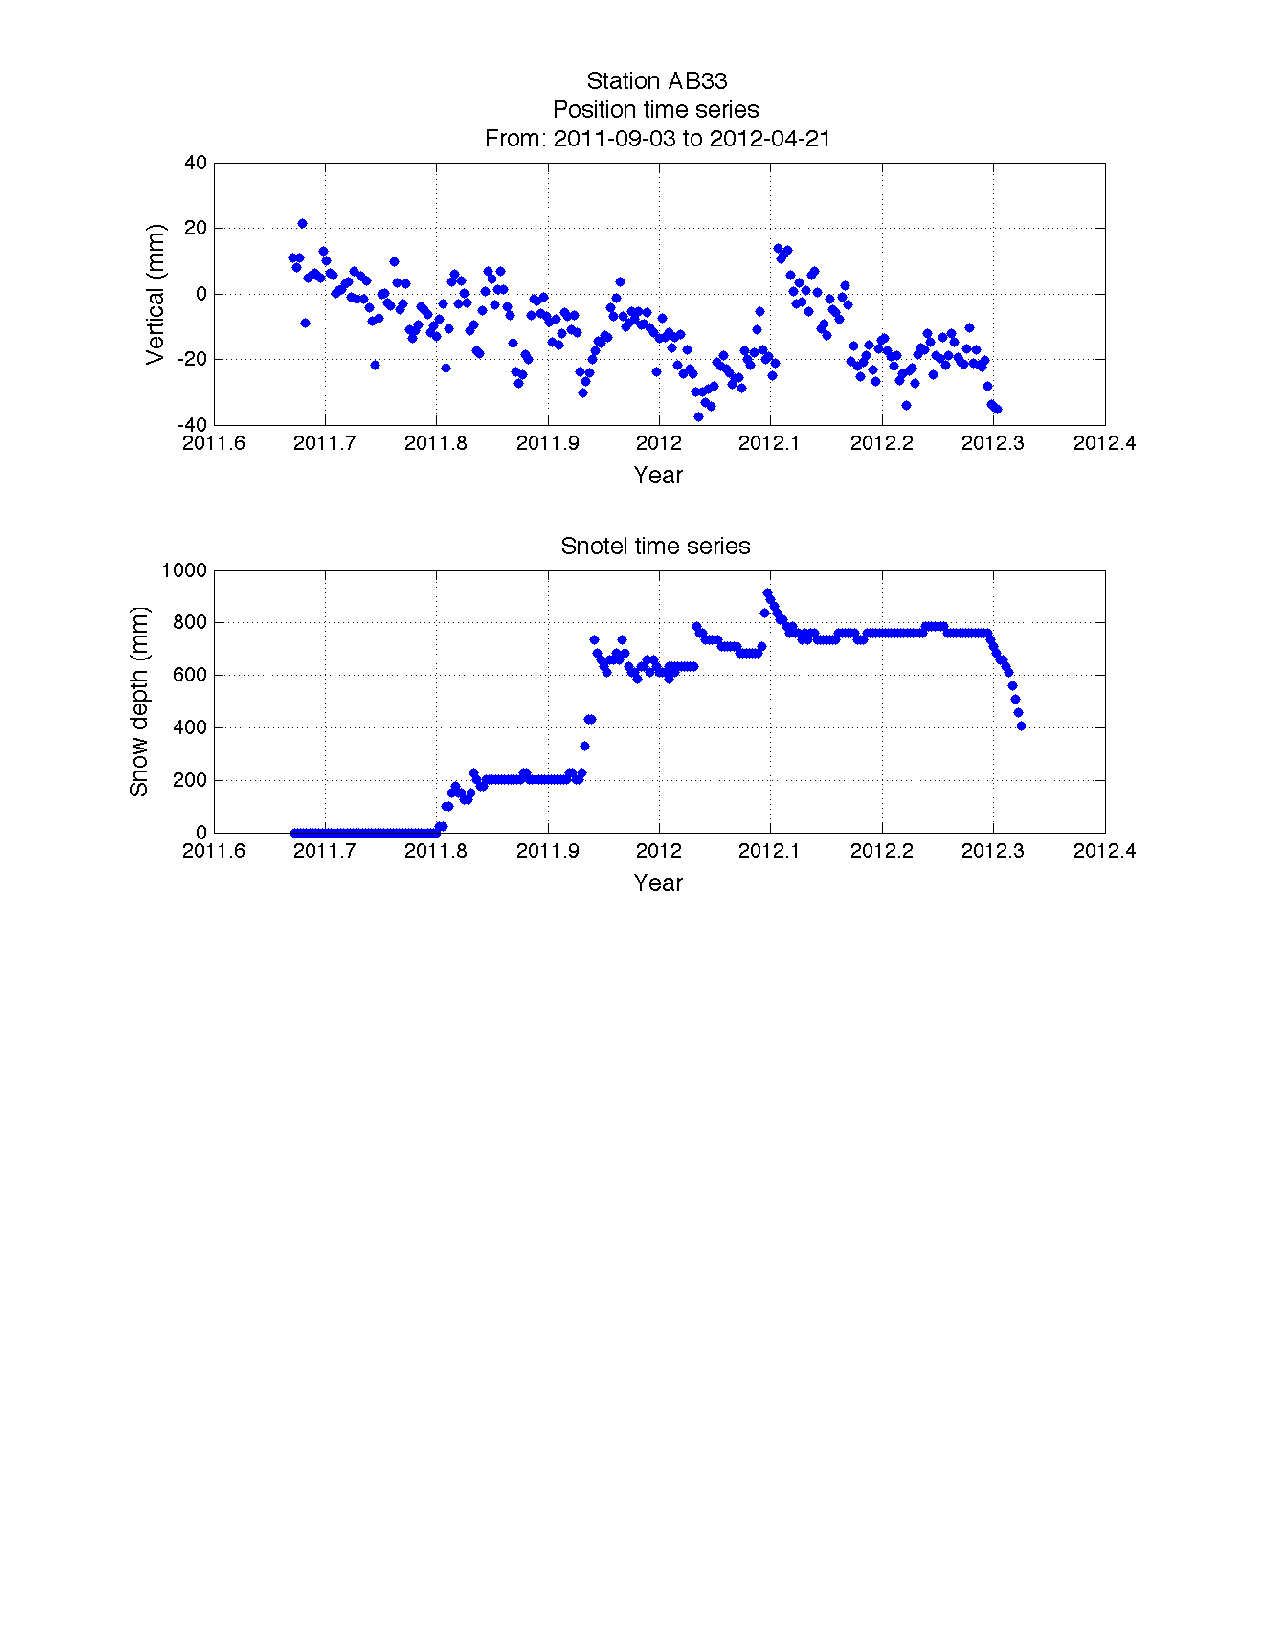
\includegraphics[width=1\linewidth,trim=50 0 50 20, clip=true]{logan/ab33_snotel.pdf}
\end{frame}

\begin{frame}{Position Time Series - P455}
\begin{itemize}
\item 2009 to 2012\\
\end{itemize}

\begin{columns}
\column{.5\textwidth}
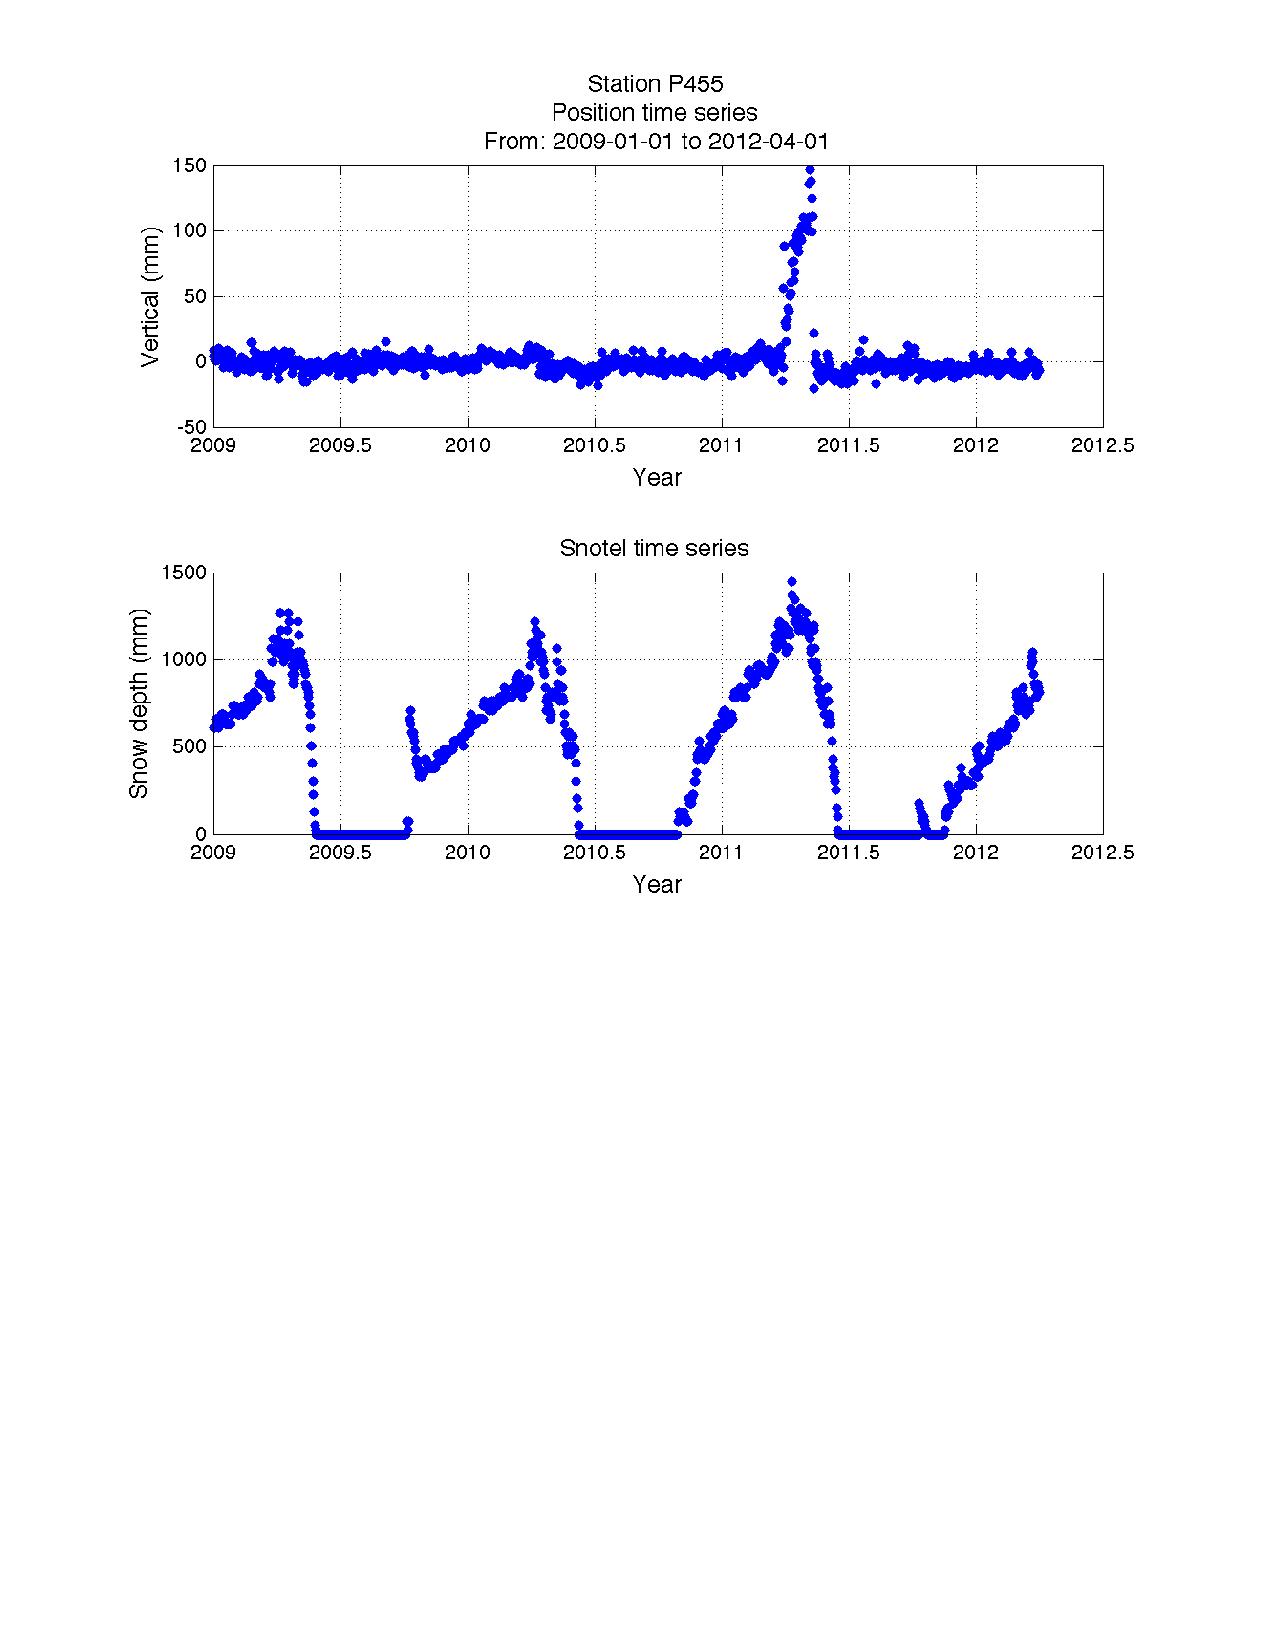
\includegraphics[width=1\linewidth,trim=70 300 70 50, clip=true]{logan/p455_pos.pdf}

\column{.5\textwidth}
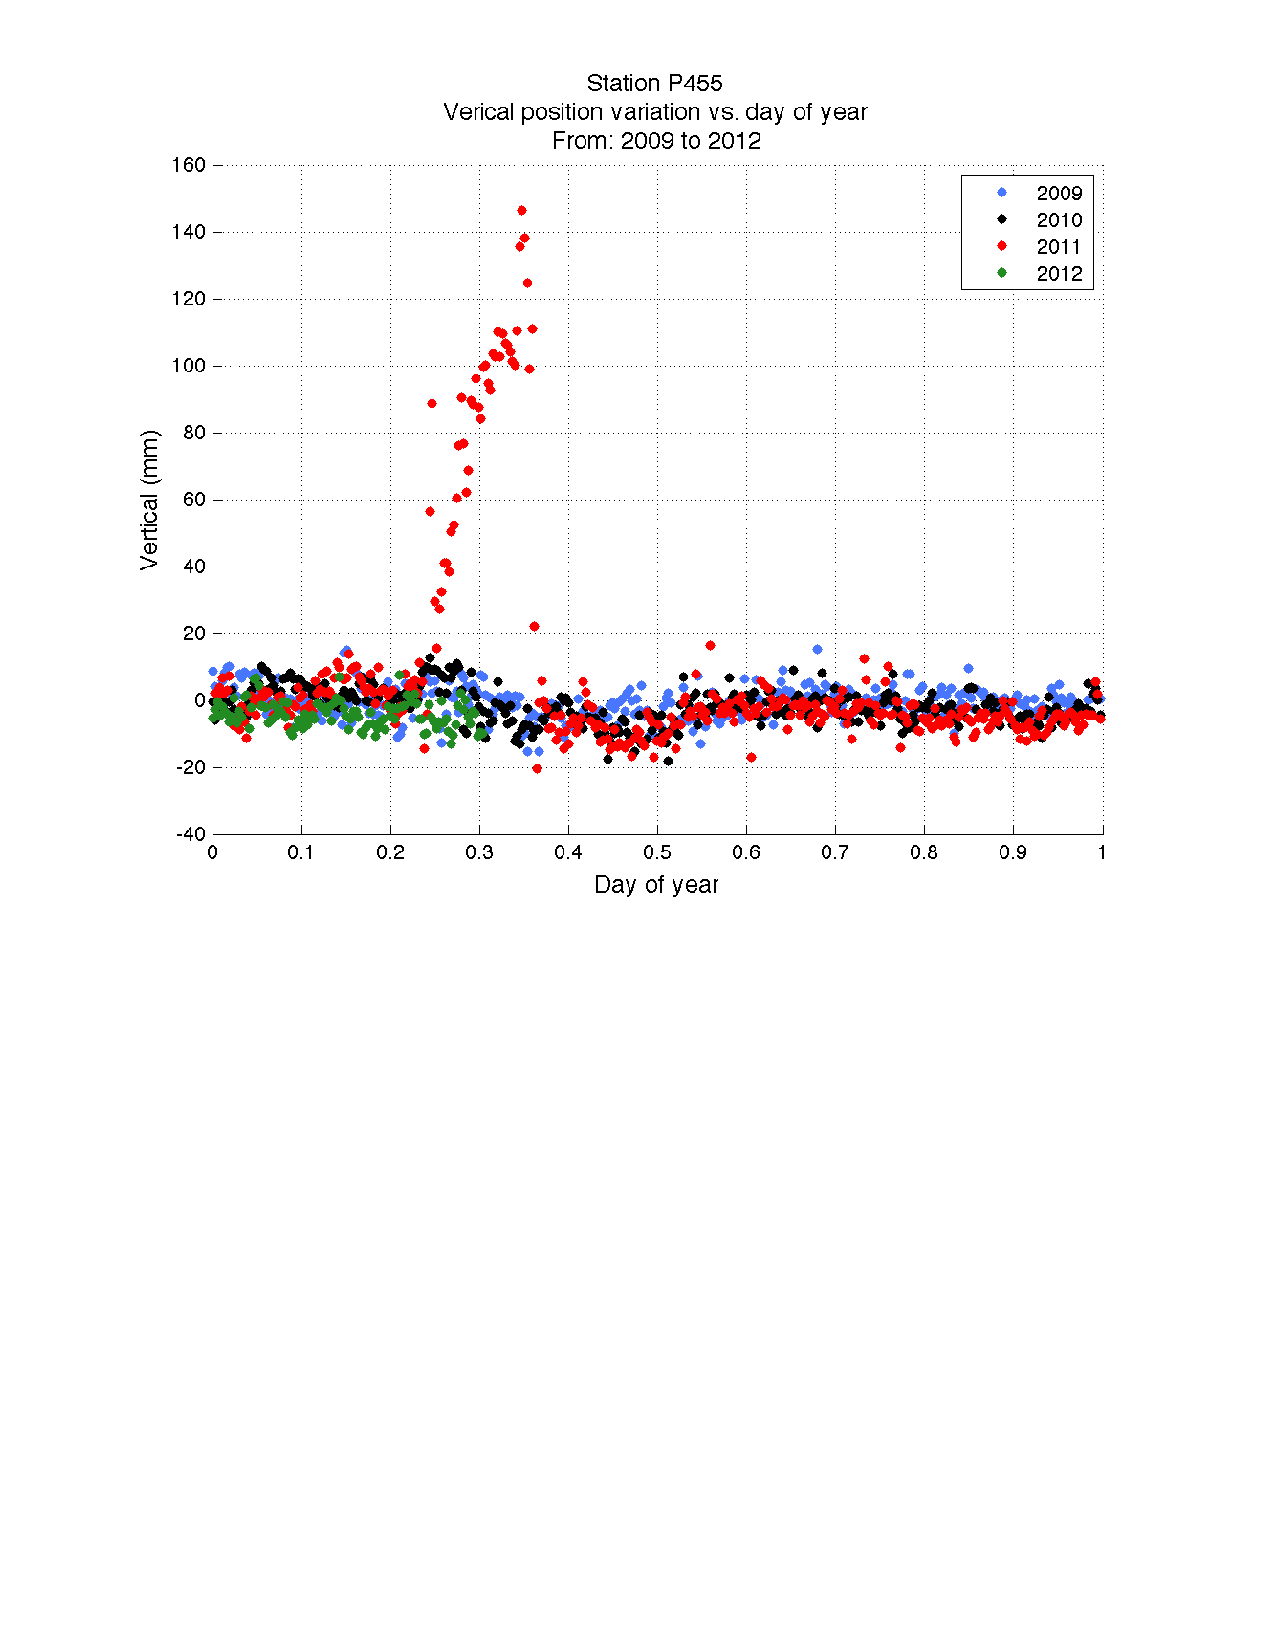
\includegraphics[width=1\linewidth,trim=70 300 70 50, clip=true]{logan/p455_pos_byYear.pdf}
\end{columns}
\end{frame}

\begin{frame}{Position Time Series - P455}
  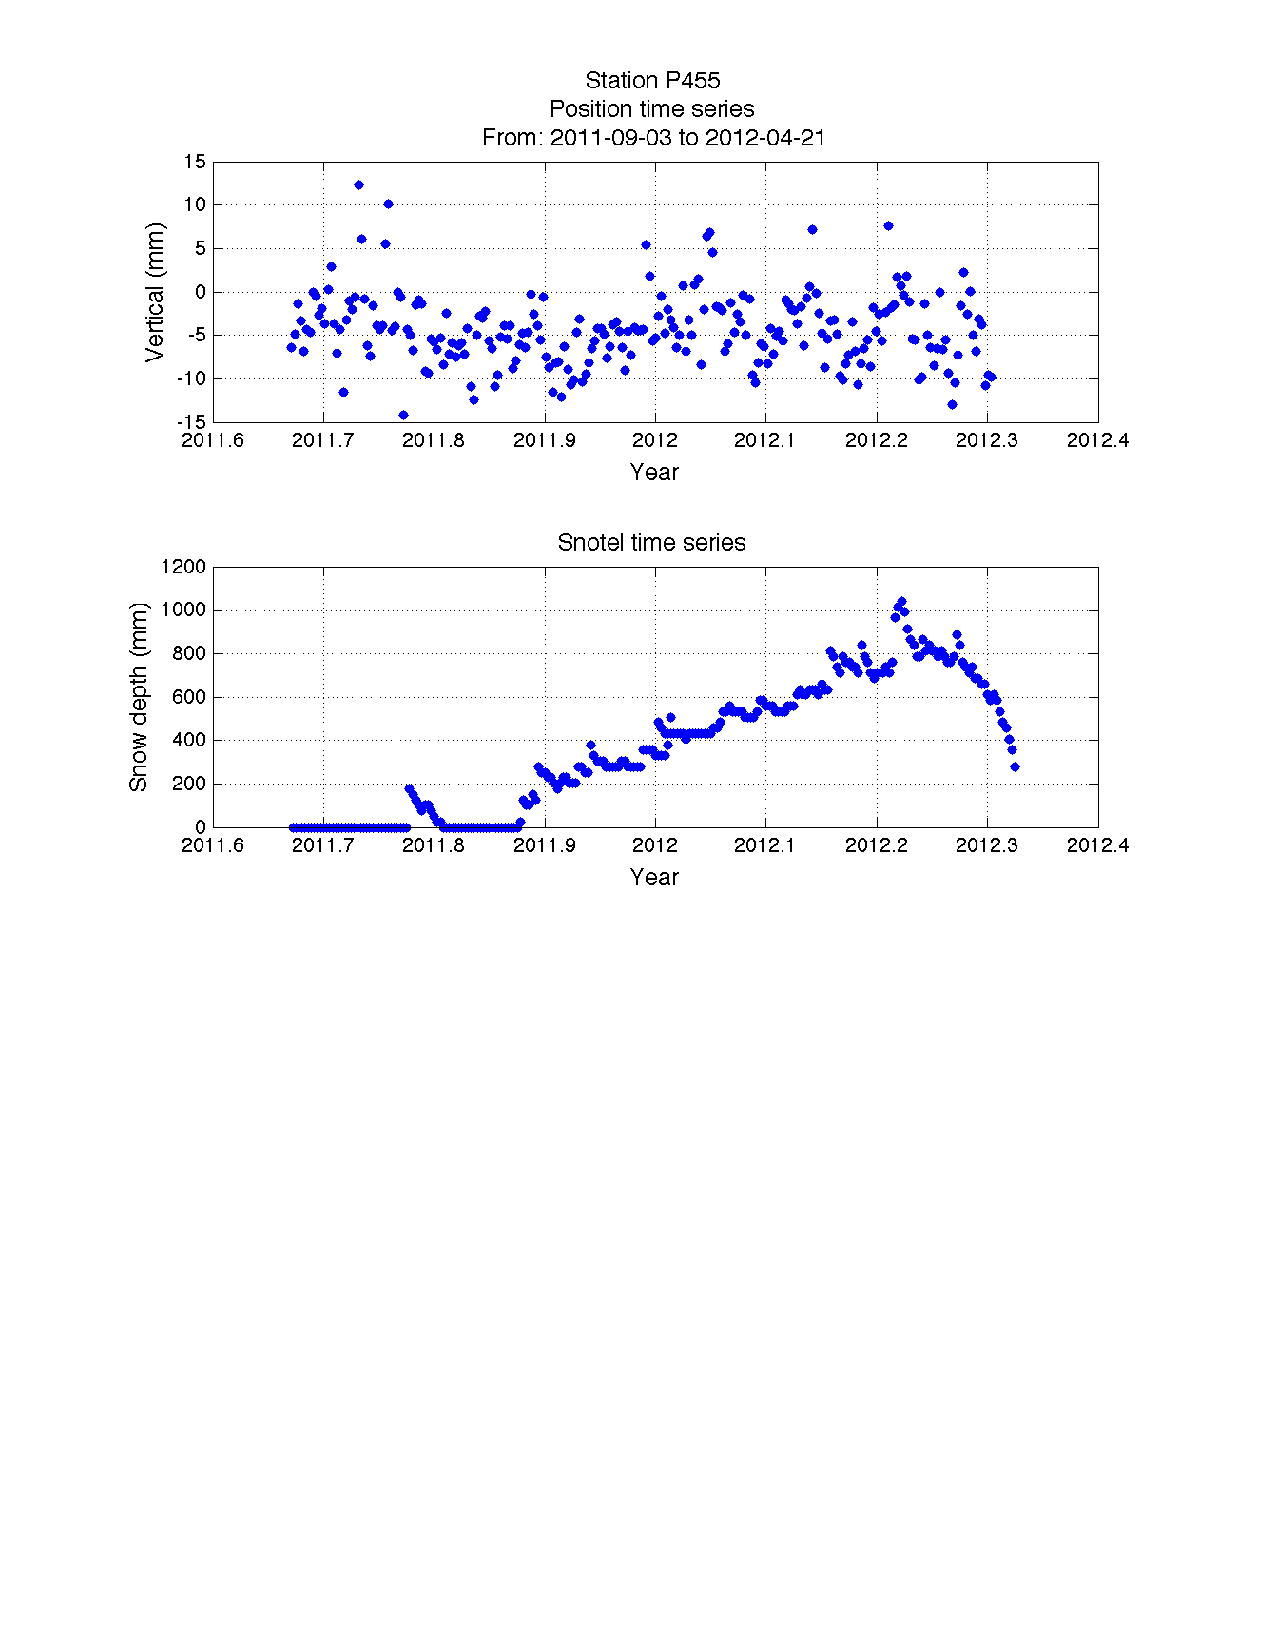
\includegraphics[width=1\linewidth,trim=50 0 50 20, clip=true]{logan/p455_snotel.pdf}
\end{frame}

\end{document}